\documentclass[border=0.5cm]{standalone}
\usepackage{tikz}
\usetikzlibrary{arrows, arrows.meta, positioning}

\tikzset{    
    disk/.style={ thick },
    traj/.style={ thin, dotted, -Latex },
    point/.style={ color=black, circle, scale=0.3, fill },
    partition/.style={ right, scale=0.75 }
}

\definecolor{light-gray}{gray}{0.9}

\def\xMin{0}
\def\xMax{9}
\def\yMin{0}
\def\yMax{5}
\def\R{0.1}

\begin{document}
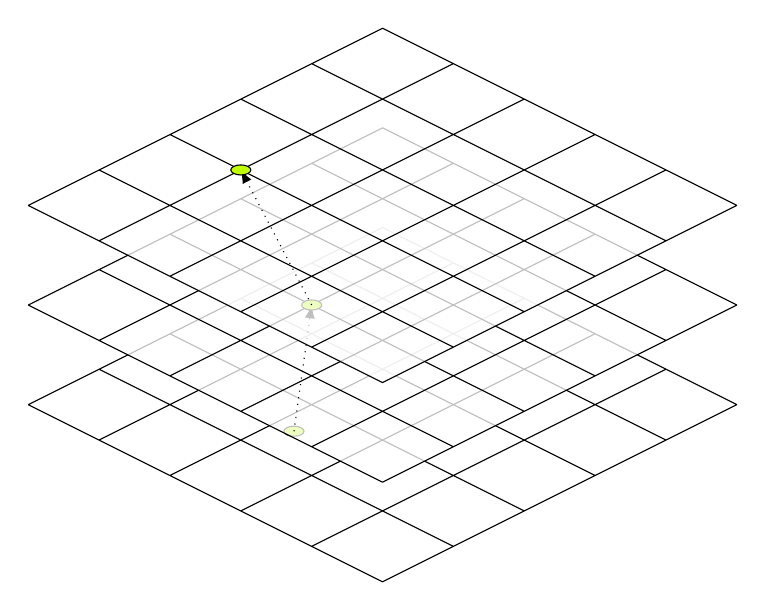
\begin{tikzpicture}[scale=.9,every node/.style={minimum size=1cm},on grid]
    %slanting: production of a set of n 'laminae' to be piled up. N=number of grids.
    \begin{scope}
        [yshift=0,every node/.append style={yslant=0.5,xslant=-1},yslant=0.5,xslant=-1]
    	\draw[step=10mm, black] (0,0) grid (5,5);
        \coordinate (A1) at (1.50, 2.75) {};
        \draw [fill=lime](A1) circle (\R) ;
        
    \end{scope}
    	
    \begin{scope}
        [yshift=40,every node/.append style={yslant=0.5,xslant=-1},yslant=0.5,xslant=-1]
        \fill[white,fill opacity=0.75] (0,0) rectangle (5,5);
        \draw[step=10mm, black] (0,0) grid (5,5);
        \coordinate (A2) at (2.00, 3.00) {};
        \draw[traj] (A1) -- (A2);
        
        \draw [fill=lime](A2) circle (\R);
    \end{scope}
    
    \begin{scope}
        [yshift=80,every node/.append style={yslant=0.5,xslant=-1},yslant=0.5,xslant=-1]
        \fill[white,fill opacity=0.75] (0,0) rectangle (5,5);
        \draw[step=10mm, black] (0,0) grid (5,5);
        \coordinate (A3) at (2.00, 4.00) {};
        \draw[traj] (A2) -- (A3);
        
        \draw [fill=lime](A3) circle (\R);
    \end{scope}
    

    %putting arrows and labels:
    %\draw[-latex,thick] (5,0) node[right]{$0$} to[out=180,in=90] (0,0);
    %\draw[-latex,thick] (5,1) node[right]{$1$} to[out=180,in=90] (0,1);
    %\draw[-latex,thick] (5,2) node[right]{$2$} to[out=180,in=90] (0,2);


\end{tikzpicture}

\end{document} 
